\documentclass[UTF8,11pt]{ctexart}
\usepackage[margin=1in]{geometry}
\usepackage{graphicx}
\usepackage{booktabs}
\usepackage{amsmath,amssymb}
\usepackage{xcolor}
\usepackage{hyperref}
\usepackage{enumitem}
\usepackage{subcaption}
\usepackage{listings}
\usepackage{tikz}
\usetikzlibrary{arrows.meta,positioning}
\hypersetup{colorlinks=true,linkcolor=blue,citecolor=blue,urlcolor=blue}
\lstset{basicstyle=\ttfamily\footnotesize,breaklines=true,columns=fullflexible,frame=single,framerule=0.3pt}

\title{面向多模态几何推理的可信校准定理路线\\
\large 精简版 arXiv Demo 报告}
\author{Anonymous Demo Draft}
\date{2026 年 6 月}

\begin{document}
\maketitle

\begin{abstract}
中间几何语言常被认为可以提升多模态大模型的几何解题能力，但我们的实验显示，这个假设并不完整。在 Geometry3K 上，把 GDP-4B 自动结构语言追加到原始图像后，并不能稳定提升 Qwen3-VL；即使是干净的 Geometry3K oracle predicates，也可能低于 image-only raw 输入。真正有用的信号更具体：当定理路线与目标量绑定时，它能修正 raw 错误；但同一个 route 通道也可能破坏原本正确的视觉答案。因此，我们把 theorem route 重新定义为“不确定干预”，而不是可信提示词。在 601 题 Geometry3K route 对比中，旧 route generator 只带来 \(+0.998\%\) 的净提升，因为它修正 40 个 raw 错误，同时破坏 34 个 raw 正确答案；compact route generator 的净提升为 \(+1.83\%\)，对应 27 个 win 和 16 个 loss。本文形式化这种 win-loss tradeoff，把理想 route gate 写成选择性风险最小化问题，并主张下一步不应继续设计更长的中间语言，而应训练能判断 route 是否与目标绑定、是否会帮助下游 MLLM 的 verifier。
\end{abstract}

\section{研究动机}
几何视觉问答要求模型读取图形、绑定标签和数值、选择定理路线，并计算目标量。因此，一个自然想法是添加中间语言，例如点线关系、结构事实或定理提示。然而，我们的结果表明，中间文本不是单调有益的。它可以补充缺失结构，也可以覆盖模型本来正确的视觉判断。

因此，本文主线收束为一个问题：
\begin{quote}
\emph{MLLM 什么时候应该相信生成的 theorem route，什么时候应该忽略它？}
\end{quote}
这个主线比“设计一种更长的中间语言”更清楚。核心证据只有三类：第一，结构语言不是 plug-and-play；第二，route 同时产生 wins 和 losses；第三，route selector 应该用反事实效果训练和评估。

\section{结构语言不是天然有效}
\begin{table}[t]
\centering
\caption{代表性结构语言实验。除纯文本 probe 外，所有条件都包含原始图像、题干和选项。}
\label{tab:structure-core-zh}
\small
\begin{tabular}{lccc}
\toprule
条件 & 正确数 & 总数 & 准确率 \\
\midrule
Geometry3K-300 raw & 158 & 300 & 52.67\% \\
Geometry3K-300 image+GDP & 154 & 300 & 51.33\% \\
Geometry3K-300 construction plan & 167 & 300 & 55.67\% \\
\midrule
Geometry3K-601 raw & 325 & 601 & 54.08\% \\
Geometry3K-601 oracle full & 318 & 601 & 52.91\% \\
Geometry3K-601 oracle top-6 cautious & 325 & 601 & 54.08\% \\
Geometry3K-601 corrupted trusted & 314 & 601 & 52.25\% \\
\bottomrule
\end{tabular}
\end{table}

\begin{figure}[t]
\centering
\begin{subfigure}{0.48\linewidth}
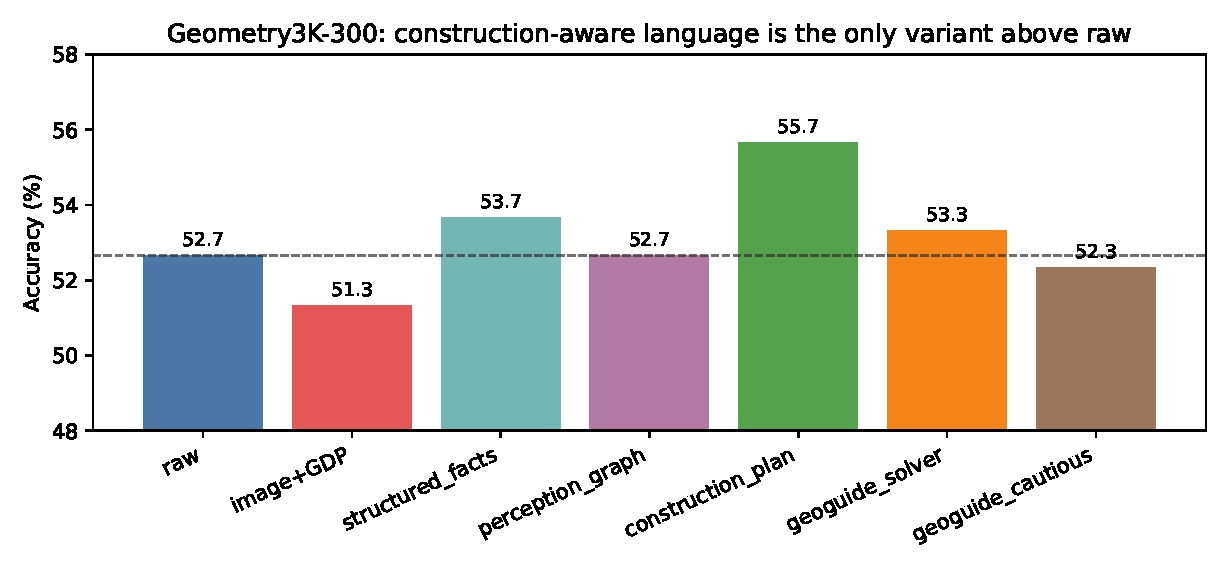
\includegraphics[width=\linewidth]{figures/main_geometry300_accuracy.pdf}
\caption{Geometry3K-300。}
\end{subfigure}\hfill
\begin{subfigure}{0.48\linewidth}
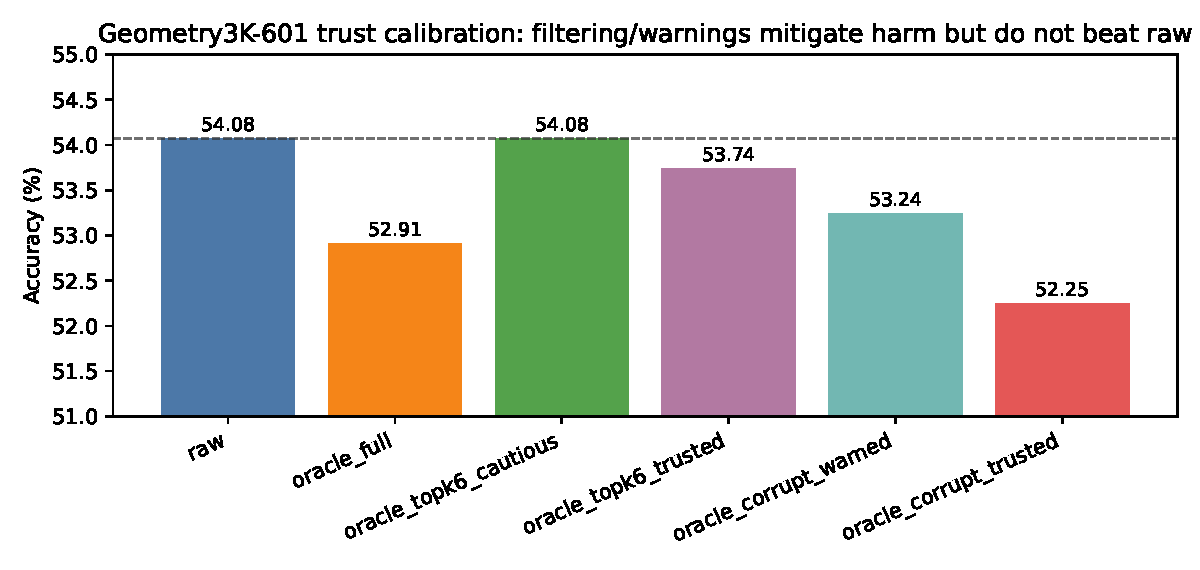
\includegraphics[width=\linewidth]{figures/trust601_accuracy.pdf}
\caption{Geometry3K-601 trust test。}
\end{subfigure}
\caption{中间结构语言并不自动有益。GDP 自动结构在 Geometry3K-300 上低于 raw；完整 oracle predicates 在 601 题测试上也低于 raw。}
\label{fig:structure-core-zh}
\end{figure}

表~\ref{tab:structure-core-zh} 说明，GDP-4B 自动结构不够可靠：在 Geometry3K-300 上，它把准确率从 52.67\% 降到 51.33\%。construction-aware oracle plan 提高到 55.67\%，但它依赖干净标注和目标条件化规则。在完整 601 题 Geometry3K 测试上，即使是 clean oracle formal predicates 也不能稳定提升 Qwen3-VL；谨慎筛选后的 top-6 oracle 版本也只是与 raw 持平。

Answer-steering 压力测试进一步说明，结构语言不是普通附加信息，而是一个高影响力控制通道。当结构文本被包装成 trusted 并指向某个答案时，MLLM 往往会跟随它。故意错误的 trusted structure 会把准确率降到 7.5\%，答案跟随率约为 90\%。

\begin{figure}[t]
\centering
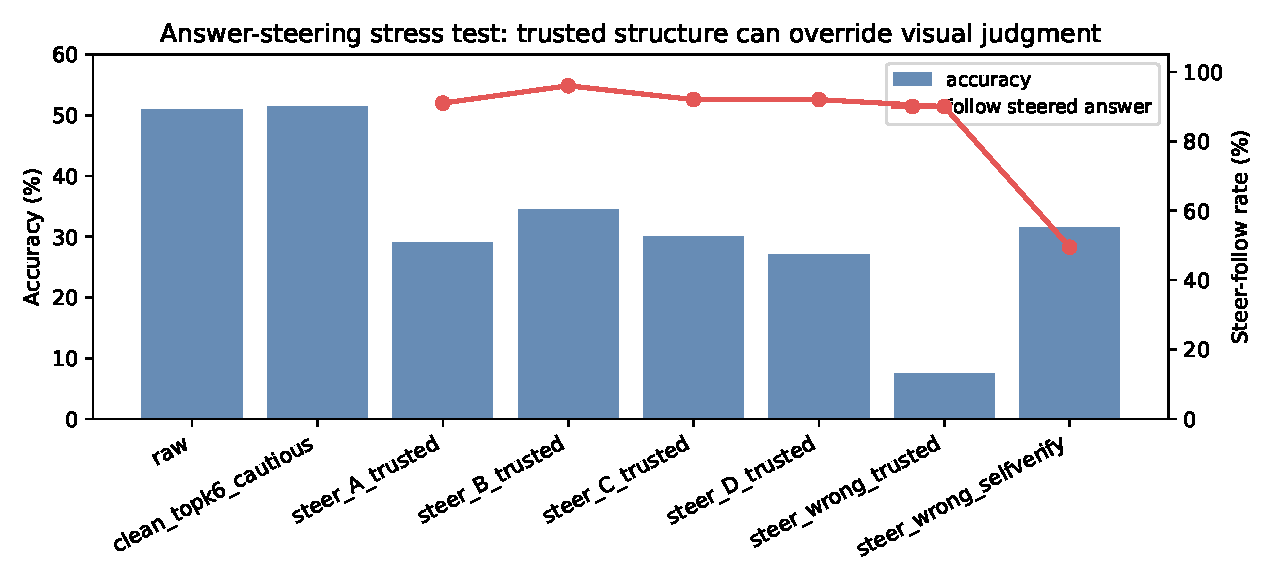
\includegraphics[width=0.75\linewidth]{figures/answer_steering.pdf}
\caption{答案诱导压力测试。被包装为 trusted 的错误结构可以压过图像和题干，因此 route 和 structure 通道必须校准。}
\label{fig:steering-core-zh}
\end{figure}

\section{定理路线有用，但也有风险}
最清楚的正向信号来自 theorem-route guidance，而不是冗长的几何事实描述。Route 是类似“使用平行对应角，然后使用相似三角形比例”的紧凑提示，不是完整解答。下游求解器仍然接收原始图像。

\begin{table}[t]
\centering
\caption{定理路线实验。Win/loss 均相对 image-only 预测计算。}
\label{tab:route-core-zh}
\small
\begin{tabular}{lcccc}
\toprule
评测 & 条件 & 准确率 & Win & Loss \\
\midrule
Geometry3K-150 & image only & 50.67\% & -- & -- \\
Geometry3K-150 & generated route & 54.67\% & 16 & 10 \\
\midrule
Geometry3K-200 & image only & 52.0\% & -- & -- \\
Geometry3K-200 & old route & 54.5\% & 15 & 10 \\
Geometry3K-200 & compact route & 56.0\% & 12 & 4 \\
\midrule
Geometry3K-601 & image only & 53.74\% & -- & -- \\
Geometry3K-601 & old route & 54.74\% & 40 & 34 \\
Geometry3K-601 & compact route & 55.57\% & 27 & 16 \\
\bottomrule
\end{tabular}
\end{table}

表~\ref{tab:route-core-zh} 支持一个更窄但更扎实的结论：定理路线可以帮助模型，但它的价值取决于修正了多少 raw 错误，以及破坏了多少 raw 正确答案。Compact route 在 601 题上比旧 route 更稳定，因为它减少了 route-induced loss。旧 generator 有时会重复同一个定理很多次，或者输出“定理本身正确但与目标无关”的路线。Compact route 通过长度约束和去重减少了这种问题，但仍然不能完全解决错误 route 和过度信任。

\section{为什么 route 效果差异很大}
\begin{figure}[t]
\centering
\begin{subfigure}{0.24\linewidth}
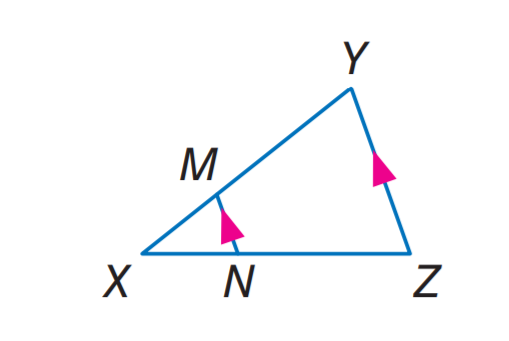
\includegraphics[width=\linewidth]{figures/route_case_2408.png}
\caption{2408：compact route 有帮助。}
\end{subfigure}\hfill
\begin{subfigure}{0.24\linewidth}
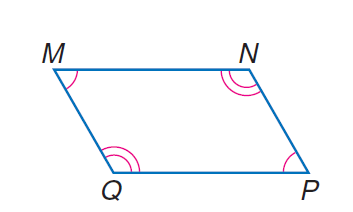
\includegraphics[width=\linewidth]{figures/route_case_2474.png}
\caption{2474：route 有害。}
\end{subfigure}\hfill
\begin{subfigure}{0.24\linewidth}
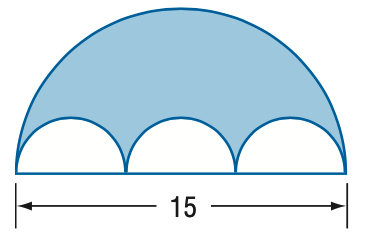
\includegraphics[width=\linewidth]{figures/route_case_2545.png}
\caption{2545：old route 有帮助。}
\end{subfigure}\hfill
\begin{subfigure}{0.24\linewidth}
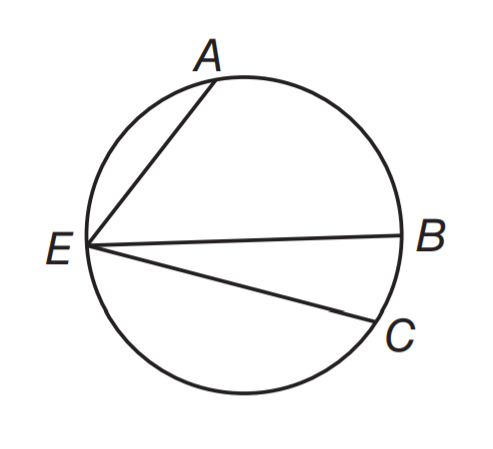
\includegraphics[width=\linewidth]{figures/route_case_2605.png}
\caption{2605：compact route 有害。}
\end{subfigure}
\caption{代表性 route 分歧案例。关键不是 route 长度，而是 route 是否绑定到目标量。}
\label{fig:route-cases-core-zh}
\end{figure}

图~\ref{fig:route-cases-core-zh} 展示了差异机制。在题 2408 中，目标是 \(NZ\)，关键关系是 \(MN\parallel YZ\)，从而得到相似三角形和比例关系。旧 route 只给“line addition”，不足以求出 \(XZ\)；compact route 指向平行角和相似三角形比例，模型答对。

题 2474 中，raw 本来正确。题目给的是平行四边形相邻角，因此需要相邻角互补；route 却强调对角相等。这个定理在平行四边形中是真的，但不是当前已知量和目标量所需的路线。这个例子说明：\textbf{theorem validity 不等于 route usefulness}。

题 2545 是另一种情况。图是多个半圆构成的阴影面积问题。old route 粗略地提示“circle area formula”，反而足以激活正确面积计算；compact route 提到了更复杂的 segment-area/power relation，和图形目标不贴合。题 2605 中，compact route 给圆角问题额外加入 external arc theorem，干扰了更简单的圆周角和角差关系。

\section{将 route 视为不确定干预}
对第 \(i\) 道题，令 \(x_i\) 表示图像、题干和选项，\(y_i\) 表示正确答案，\(r_i\) 表示生成路线，\(f_0(x_i)\) 表示 image-only 预测，\(f_r(x_i,r_i)\) 表示 route-conditioned 预测。定义 route 的反事实效应：
\begin{equation}
\Delta_i(r)=
\mathbf{1}[f_r(x_i,r_i)=y_i]
-
\mathbf{1}[f_0(x_i)=y_i].
\label{eq:route-effect-core-zh}
\end{equation}
其中 \(\Delta_i=+1\) 是 route win，\(\Delta_i=-1\) 是 route loss，\(\Delta_i=0\) 是 neutral。总体收益为：
\begin{equation}
\operatorname{Gain}(r)
=
\frac{1}{N}\sum_i \Delta_i(r)
=
\frac{W(r)-L(r)}{N}.
\label{eq:gain-core-zh}
\end{equation}
所以 old route 的收益是 \((40-34)/601=0.998\%\)，compact route 的收益是 \((27-16)/601=1.83\%\)。

Route selection 本质上是选择性预测问题。策略 \(\pi\) 在
\[
a_i\in\{\textsc{raw},\textsc{route}\}
\]
中选择一个动作，最终预测为：
\begin{equation}
\hat{y}_i=
\begin{cases}
f_0(x_i), & \pi(x_i,r_i)=\textsc{raw},\\
f_r(x_i,r_i), & \pi(x_i,r_i)=\textsc{route}.
\end{cases}
\end{equation}
理想 gate 最小化：
\begin{equation}
\min_{\pi}
\frac{1}{N}
\sum_i
\mathbf{1}[\hat{y}_i\neq y_i],
\end{equation}
并且只有当 route-conditioned 预测比 raw 更可能正确时才使用 route：
\begin{equation}
P(f_r(x_i,r_i)=y_i\mid x_i,r_i)>
P(f_0(x_i)=y_i\mid x_i).
\label{eq:optimal-gate-core-zh}
\end{equation}
这解释了为什么只判断定理“看起来合理”的 verifier 不够。Verifier 必须预测真实下游反事实：使用 route 是否比 raw 更好。

为了避免退化成提示词判断，可以定义目标绑定分数。设几何图为 \(G_i=(V_i,E_i,R_i)\)，目标量为 \(\tau_i\)。Route \(r_i=(t_1,\ldots,t_K)\) 中每个定理有前提 \(\mathcal{P}_k\) 和结论 \(\mathcal{Q}_k\)。一个简单的绑定分数为：
\begin{equation}
B(r_i,\tau_i,G_i)
=
\lambda_1\operatorname{cov}\!\left(\tau_i,\bigcup_k\mathcal{Q}_k\right)
+\lambda_2\operatorname{cov}\!\left(K_i,\bigcup_k\mathcal{P}_k\right)
-\lambda_3\operatorname{miss}(r_i,G_i),
\label{eq:binding-core-zh}
\end{equation}
其中 \(K_i\) 是题干已知量。该分数奖励结论触达目标、前提使用已知量、对象被图像或 parse 支持的 route。

最后，设 \(p_h\) 是 route 修正 raw 错误的概率，\(p_c\) 是 route 破坏 raw 正确答案的概率，则：
\[
\mathbb{E}[\Delta]=p_h-p_c.
\]
若 gate 接受 helpful route 的概率为 \(\alpha\)，错误接受 harmful route 的概率为 \(\beta\)，则：
\begin{equation}
\mathbb{E}[\Delta_{\text{gate}}]
=
\alpha p_h-\beta p_c,
\qquad
\text{有效 gating 需要}\quad
\frac{\alpha}{\beta}>
\frac{p_c}{p_h}.
\label{eq:harm-condition-core-zh}
\end{equation}
之前 verifier 没有明显提升，可以理解为没有充分降低 \(\beta\)：很多 harmful route 在表面上仍然像合理定理。

\section{哪些内容应删除或后置}
长版 demo 中有些实验对开发有用，但不适合作为主论文核心。GDP-to-construction-plan generator 在 200 题上只有 \(+1.0\) 个百分点的小幅收益，更像 preliminary engineering attempt。FormalGeo partial checkpoint 不应作为主结果出现，除非完整实验结束。MathVista transfer 可以作为边界条件，但会分散本文“几何定理路线可信校准”的主线。这些内容更适合放到附录，或暂时从主稿删除。

\section{下一步}
下一步应训练 target-binding route verifier，并用反事实标签监督：
\[
\text{raw wrong, route correct}\rightarrow \textsc{use\_route},
\qquad
\text{raw correct, route wrong}\rightarrow \textsc{reject\_route}.
\]
Hard negatives 应该是“局部看起来合理但目标不匹配”的路线，例如平行四边形题中使用真实但不服务当前相邻角方程的定理。评测也不应只报告 accuracy，还应报告 win、loss、route acceptance rate 和 route-helpfulness confidence 的校准情况。

\section{结论}
核心结论不是“中间几何语言总能提升 MLLM”。相反，很多结构语言并不能提升，甚至会伤害模型。更强的结论是：定理路线只有作为可信校准的不确定干预时才有价值。Compact route 在 Geometry3K 上提升 Qwen3-VL，是因为它减少了 route-induced loss，同时保留了足够的 route-induced win。下一步真正有研究价值的贡献应是 target-binding verifier 和 counterfactual evaluation protocol，而不是继续设计更长的 prompt 格式。

\end{document}
